\chapter{Výsledky testů}
\label{chap:results}

\section{Výsledky subjektivních testů}

Nakonec byly oba testy představené v kapitole \ref{chap:realization} provedeny sedmnácti subjekty ve věkovém intervalu od 21 do 62 let. Šest z nich mělo předchozí zkušenosti s poslechovými testy. Poměr mužských posluchačů vůči ženám byl přibližně 2:1. Všem byly poskytnuty průvodní informace, prošli fází zaučení a podepsali informovaný souhlas. 

Dvě formy post-screeningu byly aplikovány na množinu získaných hodnocení. První za pomoci skryté reference a druhá pomocí skryté kotvy. Doporučení říká, že subjekty jejichž hodnocení skryté reference je v patnácti procentech případů nižší než devadesát procent, by měli být vyřazeni. To je poměrně přísná podmínka a při jejím aplikování by bylo vyřazeno více než 60 \% subjektů. Protože test míří na běžné posluchače rozhlasového vysílání, nikoliv na studiový poslech znalými posluchači, bylo toto kritérium poníženo a vyřazeni byli ti, jejichž průměrné hodnocení vzorků bylo nižší než 90 \%. Zároveň nejsou zahrnuta hodnocení posluchačů, jejichž průměrné hodnocení skryté kotvy bylo vyšší než 50 \%. Prvním kritériem byly vyřazeni tři posluchači a druhým jeden další. Celkový počet subjektů s relevantním hodnocením byl tedy roven $N = 12$.

Výsledky poslechových testů jsou vyneseny do tabulek \ref{table:mos:test1} a \ref{table:mos:test2}. Zároveň jsou vyobrazeny pomocí sloupcových grafů, které ukazují průměr subjektivně vnímané poslechové kvality $\overline{u}_{jk}$. Na obrázcích \ref{pic:mushra1} a \ref{pic:mushra2} lze vidět průměrné hodnocení přes všechny zkoušky. Grafy \ref{pic:mushra1:kat} a \ref{pic:mushra2:kat} tyto hodnoty dělí do třech sledovaných kategorií: hudební, řečové a smíšené. Všechny výsledky jsou doplněny chybovými úsečkami vyznačující interval spolehlivosti o velikosti $2\delta_k$ vypočítaný podle vztahu \ref{equation:inteval}, ve kterém se s 95\% pravděpodobností nachází populační průměr. 

\begin{table}[h]
\centering
\begin{tabular}{|c|c|c|c|c|c|c|c|c|c|c|c|}
\hline
 & \rot{128 MP2} & \rot{24 opus} & \rot{32 HE-AAC v2} & \rot{32 opus} & \rot{48 HE-AAC v1} & \rot{48 HE-AAC v2 } & \rot{64 HE-AAC v1} & \rot{64 LC-AAC} & \rot{96 MP2} & \rot{hidden ref} & \rot{lp35}\\ \hline
$\overline{u}_{k}$ & 82,3 & 59,4 & 26,6 & 67,3 & 58,1 & 62,6 & 85,0 & 86,4 & 18,7 & 96,6 & 11,9 \\ \hline
$\delta_{k}$ & 8,1 & 6,9 & 3,7 & 6,7 & 8,5 & 7,5 & 9,0 & 8,4 & 5,4 & 1,9 & 6,8 \\ \hline
$\overline{u}_{jk(music)}$ & 78,2 & 42,2 & 19,7 & 60,0 & 51,1 & 54,7 & 84,8 & 85,6 & 13,3 & 96,8 & 11,5 \\ \hline
$\delta_{jk(music)}$ & 9,0 & 7,2 & 3,2 & 5,2 & 7,2 & 10,0 & 9,8 & 9,4 & 5,7 & 1,6 & 7,6 \\ \hline
$\overline{u}_{k(speech)}$ & 89,0 & 86,7 & 45,8 & 73,5 & 72,4 & 80,1 & 97,0 & 95,4 & 34,3 & 95,9 & 14,3 \\ \hline
$\delta_{k(speech)}$ & 10,5 & 7,0 & 11,7 & 10,9 & 16,2 & 8,8 & 3,1 & 4,5 & 14,1 & 4,3 & 11,4 \\ \hline
$\overline{u}_{k(mixed)}$ & 88,0 & 84,0 & 28,0 & 83,0 & 64,7 & 68,8 & 73,4 & 80,1 & 19,4 & 96,7 & 10,4 \\ \hline
$\delta_{k(mixed)}$ & 6,5 & 9,1 & 7,6 & 12,4 & 11,6 & 10,7 & 19,6 & 16,6 & 10,2 & 2,4 & 9,5 \\ \hline
\end{tabular}
\caption{Výsledky prvního testu}
\label{table:mos:test1}
\end{table}

\begin{figure}[h!]
    \centering
    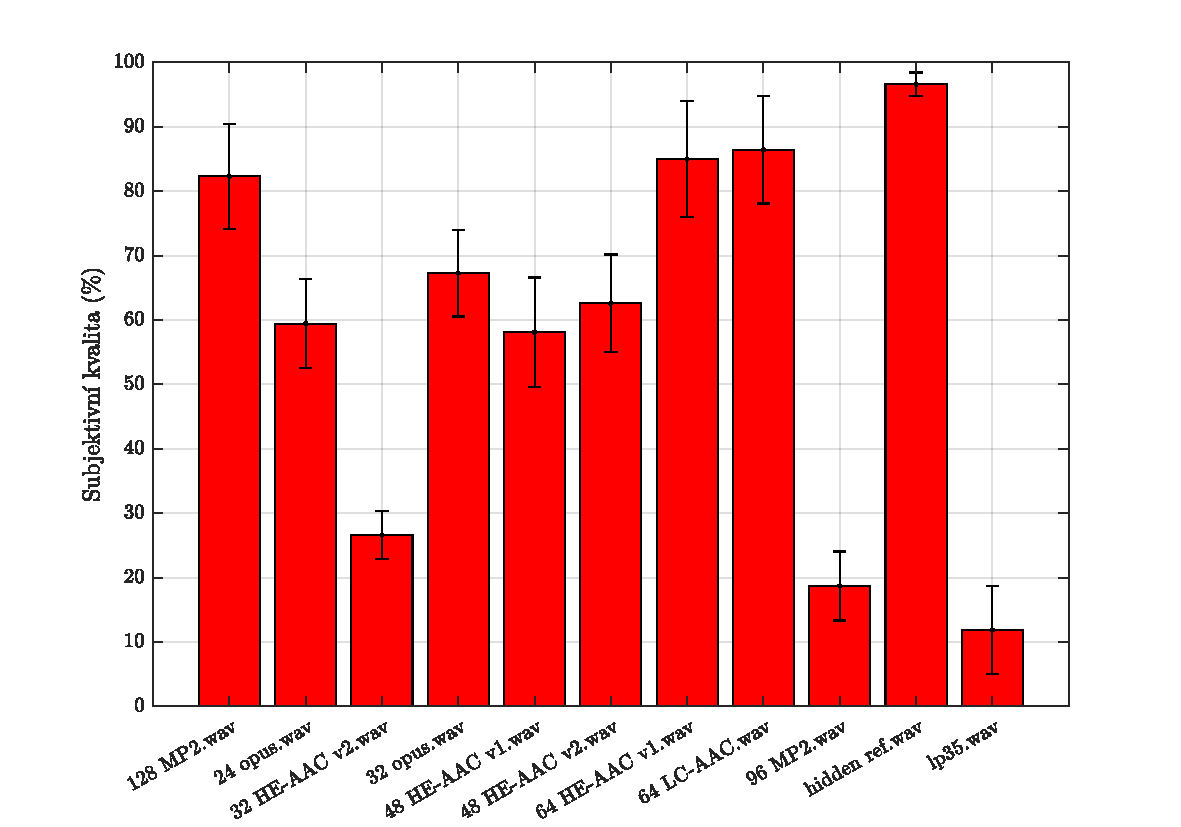
\includegraphics[width = 1\textwidth]{pic/mushra1Mean.pdf}
    \caption{Grafické zobrazení výsledků prvního testu}
    \label{pic:mushra1}
\end{figure}

\begin{figure}[h!]
    \centering
    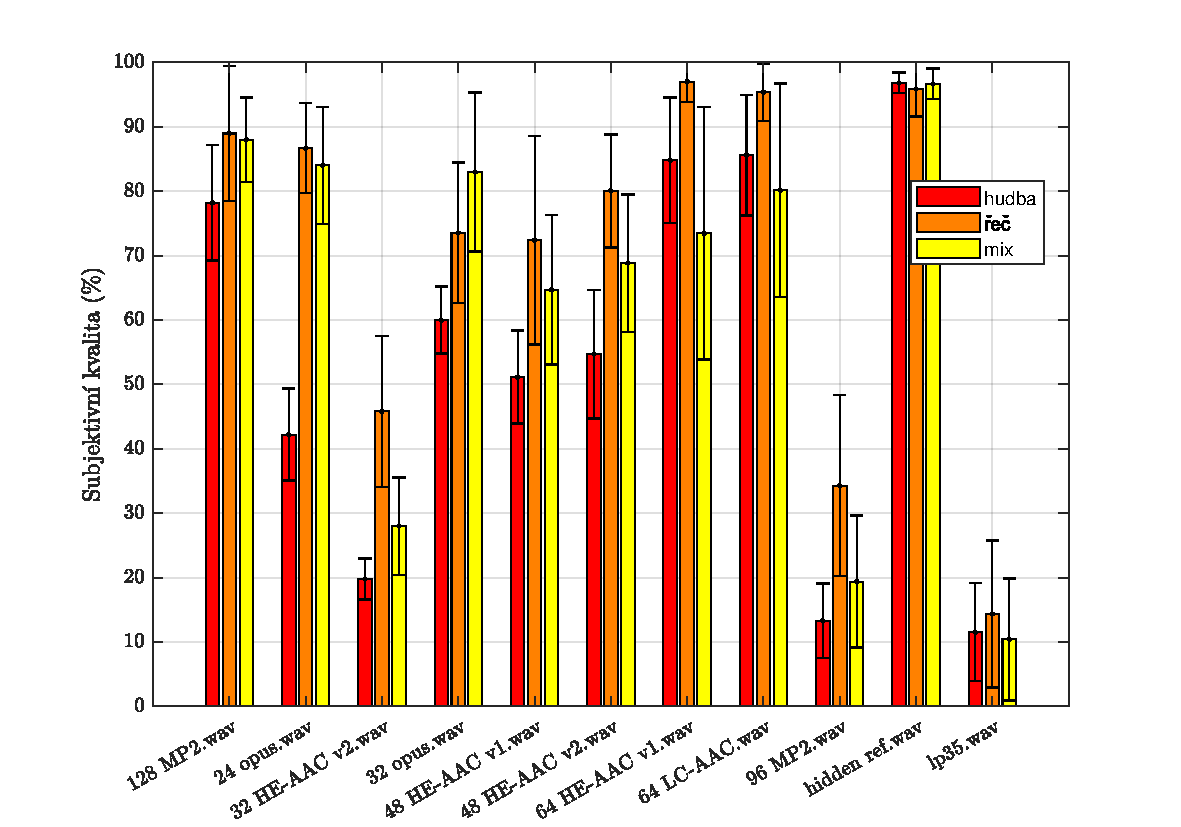
\includegraphics[width = 1\textwidth]{pic/mushra1.pdf}
    \caption{Grafické zobrazení výsledků prvního testu rozdělené do kategorií}
    \label{pic:mushra1:kat}
\end{figure}


\begin{table}[h]
\centering
\begin{tabular}{|c|c|c|c|c|c|c|c|c|c|}
\hline
 & \rot{12 Opus} & \rot{12 xHE-AAC} & \rot{24 HE-AAC v2} & \rot{24 Opus} & \rot{48 HE-AAC v2} & \rot{64 HE-AAC v2 } & \rot{8 xHE-AAC} & \rot{hidden} & \rot{lp35} \\ \hline
$\overline{u}_{k}$ & 24,7 & 48,2 & 27,8 & 68,6 & 61,0 & 65,5 & 28,5 & 97,1 & 16,0 \\ \hline
$\delta_{k}$ & 8,0 & 11,1 & 10,3 & 6,1 & 15,0 & 6,7 & 11,9 & 2,5 & 8,9 \\ \hline
$\overline{u}_{jk(music)}$ & 14,3 & 57,0 & 31,3 & 53,6 & 58,6 & 59,5 & 43,3 & 95,1 & 13,6 \\ \hline
$\delta_{jk(music)}$ & 11,1 & 25,6 & 12,6 & 17,0 & 23,3 & 18,3 & 20,5 & 6,2 & 7,7 \\ \hline
$\overline{u}_{k(speech)}$ & 40,9 & 68,2 & 25,1 & 82,0 & 68,3 & 68,3 & 29,5 & 97,8 & 24,3 \\ \hline
$\delta_{k(speech)}$ & 12,5 & 18,1 & 11,9 & 7,0 & 14,1 & 15,3 & 13,3 & 2,1 & 13,8 \\ \hline
$\overline{u}_{k(mixed)}$ & 18,9 & 19,4 & 26,8 & 70,3 & 56,0 & 68,7 & 12,8 & 98,4 & 10,2 \\ \hline
$\delta_{k(mixed)}$ & 9,9 & 7,5 & 11,0 & 14,1 & 12,1 & 9,2 & 9,1 & 2,2 & 8,3 \\ \hline
\end{tabular}
\caption{Výsledky druhého testu}
\label{table:mos:test2}
\end{table}

\begin{figure}[h!]
    \centering
    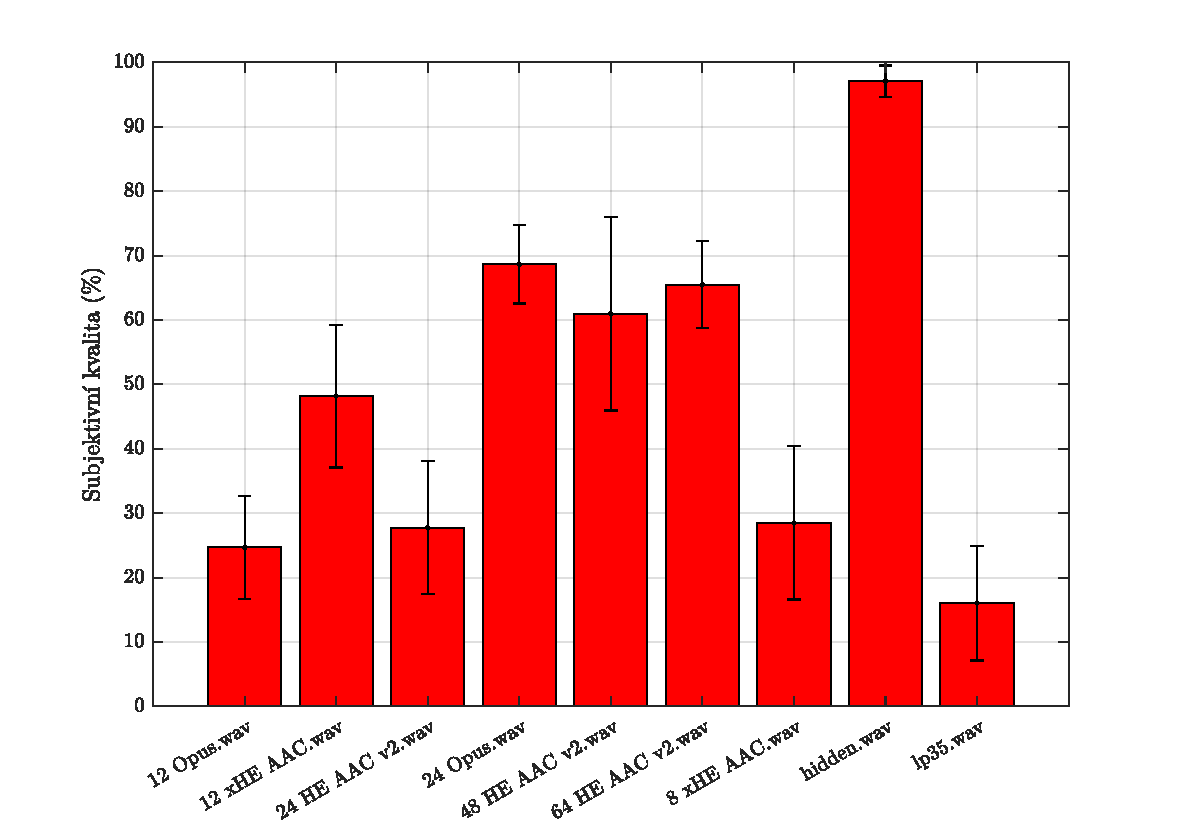
\includegraphics[width = 1\textwidth]{pic/mushra2Mean.pdf}
    \caption{Výsledky testu MUSHRA pro nižší bitové rychlosti}
    \label{pic:mushra2}
\end{figure}

\begin{figure}[h!]
    \centering
    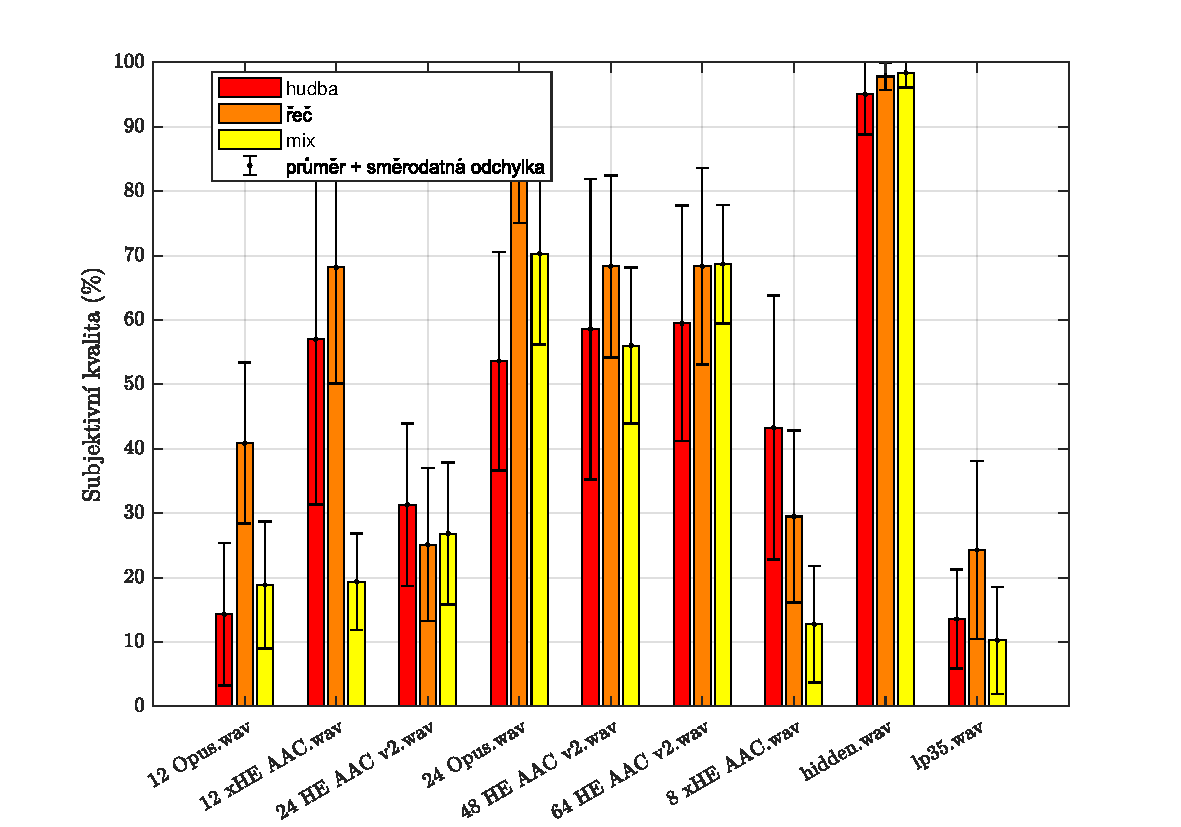
\includegraphics[width = 1\textwidth]{pic/mushra2.pdf}
    \caption{Výsledky testu MUSHRA pro nižší bitové rychlosti včetně kategorií}
    \label{pic:mushra2:kat}
\end{figure}

Jako ukazatel výpovědní hodnoty dosažených výsledků lze brát shodu v hodnocení vzorků konzistentních pro oba testy (zeleně vyznačených v tabulkách \ref{table:test1} a \ref{table:test2}). Průměrné hodnocení stimulů zakódovaných kodekem HE-AAC v2 o bitové rychlosti 48 kb/s dosáhlo hodnot $\overline{u} = 62,6 \%$ s velikostí intervalu spolehlivosti $2\delta = 15 \%$ pro první test a $\overline{u} = 61 \%$ v intervalu s velikostí $2\delta = 30 \%$ pro test druhý. Druhý set vzorků určených pro kontrolu hodnocení mezi dvěma testy byl zkomprimován kodekem Opus s bitovou rychlostí 24 kb/s. Průměrné hodnocení posluchačů v prvním testu $\overline{u} = 59,4 \%$ na intervalu $2\delta = 13,8 \%$ se s průměrnou hodnotou získanou druhým testem $\overline{u} = 68,4 \%$ na intervalu $2\delta = 12,2 \%$ shoduje o něco méně než v prvním případě, se stále však jedná o srovnatelné hodnoty.

Nejlepší hodnocení získala v obou testech skrytá reference a nejhorší skrytá kotva. MPEG Layer II na 96 kb/s dopadl jen o málo lépe než signál omezený dolní propustí o nominálním kmitočtu 3,5 kHz, jelikož při nedostatečné bitové rychlosti jeho psychoakustický model poměrně agresivně kvantizuje vyšší kmitočty a chová se tak jako dolní propust.

Mezigenerační souboje členů rodiny AAC naznačují, že použití metody \textit{Spectral Band Replication} na rychlosti 64 kb/s nepřináší významné vylepšení subjektivně vnímané kvality. Její růst o pár procentních bodů na hodnotící škále lze ovšem sledovat na rychlosti 48 kb/s při použití parametrického sterea. Při poklesu bitové rychlosti na 32/kb už ovšem kvalita padá do oblasti označené jako \uv{špatná}. Proti tomu kodek Opus na stejných rychlostech dosahuje výsledků o zhruba jednu až dvě kvalitativní úrovně výše.

S výjimkou kodeku Opus, u kterého na vyšších rychlostech dopadají nejlépe smíšené vzorky, hodnotí posluchači hudební vzorky hůře než nahrávky z kategorií mluvené slovo a smíšené vzorky. Řeč je ovšem z frekvenčního hlediska méně komplexní než hudba a tak se u ní projevují kompresní artefakty ve srovnání se zakódovanou hudbou méně, i při použití kodeků které nejsou přímo určené ke kompresi mluveného slova. Při započítání překryvů intervalů spolehlivosti dosahují rozdíly v hodnocení jednotlivých kategorií maximálně deseti procent. Celkově se dá pozorovat, že s klesající bitovou rychlostí roste rozptyl získaných hodnot. V testu na nižších bitových rychlostech dosahuje velikost intervalu spolehlivosti hodnoty až $ 2\delta = 30 \%$.

Co druhý test nepotvrdil je výhoda sjednoceného kódování řeči a hudby profilem xHE-AAC. U obou testovaných bitových rychlostí dopadl smíšený vzorek nejhůře ze všech třech kategorií a to s více než desetiprocentní ztrátou oproti průměrné hodnotě. U kodeku Opus dopadají nejlépe téměř výhradně vzorky řečové. Celkově ale xHE-AAC dosahuje vyšší kvality při nízkých rychlostech ve srovnání s ostatními použitými kodeky.

Pokud by tento test měl sloužit jako výběr ideálního kandidáta pro přenos signálu digitálním rádiem, nebyl by zřejmě příliš úspěšný, neboť jen minimum vzorků dosahuje úrovně \uv{Vynikající} či \uv{Dobrá}. Spíše se výsledky pohybují od hladiny 80 \% níže, až po úroveň označovanou jako nedostatečná. Toto \uv{rozprostření} výsledků přes všechny možné úrovně se však hodí pro porovnávání výsledků získaných objektivními algoritmy. Zvýší se tím výpovědní hodnota grafů v následující podkapitole.


\section{Porovnání objektivních a subjektivních výsledků}

Při určování věrohodnosti objektivních metod jsou brány výsledky subjektivních testů jako referenční ukazatel kvality. Při výpočtech a zobrazení je počítáno s aritmetickým průměrem hodnot subjektivně vnímané kvality přes množinu všech subjektů. Všemi předem zmíněnými algoritmy byl za pomocí skriptů popsaných v kapitole \ref{chap:realization} ohodnocen stejný set vzorků jako při poslechových testech. Grafy na obrázku \ref{fig:compare} zobrazují závislost hodnocení kvality objektivními algoritmy na subjektivně vnímané kvalitě pro jednotlivé hodnotící metody. Po vzoru článku \textit{Objective Assessment of Perceptual Audio Quality Using ViSQOLAudio} \cite{article:assessment} byly výsledky všech testů přepočítány na stejnou míru, respektive zobrazeny na stejné škále, aby bylo porovnání přehledné a objektivní. U subjektivních testů byla lineární sto-dílková škála $CQS$ jednoduchým vydělením přepočtena na $SDG$. PEAQ a PEMO-Q poskytují výsledky ve formě $ODG$ a na tu byly přepočítány i výsledky algoritmu ViSQOL, přepočtem z jeho standardního výstupu $MOS\text{-}LQO$. Barevně a za pomocí znaků jsou v nich odlišené metody komprese. Těm je rovněž přidělená eliptická oblast, kde poloosa ve vodorovném směru odpovídá směrodatné odchylce výsledků subjektivních testů a svislá poloosa odpovídá směrodatné odchylce objektivních hodnocení zároveň uvedených v tabulce \ref{table:sigma}. 

Jelikož ideální případ závislosti $ODG$ na $SDG$ je jejich rovnost (čerchovaná modrá přímka) lze velikost chyby spočítat jejich rozdílem. Z těchto rozdílů lze vypočítat střední kvadratickou chybu $\varepsilon$ (\textit{Root Mean Squared Error}) podle:

\begin{equation}
    {\varepsilon} = \sqrt{\sum_{j=1}^{J}\frac{({ODG_j}-{SDG_j})^2}{J}}
\end{equation}

V tabulce \ref{table:epsilon} je vypočítané $\varepsilon$ pro všechny testované metody komprese pomocí všech objektivních metod a v tabulce \ref{table:epsilon:avg} jsou průměrné hodnoty $\overline{\varepsilon}$ a průměru kodeků používaných v digitálním rádiu $\overline{\varepsilon}_{radio}$.

\tabulinesep=1.3mm
\begin{table}[h]
\centering
\small
\begin{tabu}{|c|c|c|c|c|c|c|c|c|c|c|c|c|c|}
\hline
 & \rot{128 MP2} & \rot{24 opus} & \rot{32 HE-AAC v2} & \rot{32 opus} & \rot{48 HE-AAC v1} & \rot{48 HE-AAC v2 } & \rot{64 HE-AAC v1} & \rot{64 LC-AAC} & \rot{96 MP2} & \rot{8 xHE AAC} & \rot{12 xHE AAC} & \rot{lp35} & \rot{uncompressed} \\ \hline
$\varepsilon_{\text{peaq-a.}}$ & 1,70 & 0,70 & 0,46 & 1,34 & 1,16 & 1,27 & 1,49 & 1,79 & 0,40 & 1,62 & 0,75 & 0,21 & 0,15 \\ \hline
$\varepsilon_{\text{peaq-b.}}$ & 1,19 & 0,99 & 0,45 & 1,23 & 0,96 & 0,35 & 1,31 & 1,77 & 0,42 & 1,61 & 0,63 & 0,57 & 0,15 \\ \hline
$\varepsilon_{\text{pemoq}}$ & 0,46 & 0,48 & 0,45 & 1,67 & 1,04 & 0,99 & 0,97 & 1,30 & 1,02 & 1,68 & 0,73 & 1,19 & 0,15 \\ \hline
$\varepsilon_{\text{visqol}}$ & 0,66 & 1,30 & 1,03 & 0,58 & 0,48 & 0,35 & 0,92 & 1,02 & 1,64 & 1,21 & 0,98 & 0,99 & 0,15 \\ \hline
\end{tabu}
\caption{Kvadratické střední chyby $\varepsilon$ pro jednotlivé kompresní metody}
\label{table:epsilon}
\end{table}

\begin{table}[h]
\centering
\begin{tabu}{|c|c|c|}
\hline
 & $\overline{\varepsilon}$ & $\overline{\varepsilon}_{radio}$ \\ \hline
PEAQ A. & 1,01 & 1,27 \\ \hline
PEAQ B. & 0,89 & 1,04 \\ \hline
PEMO-Q & 0,87 & 1,01 \\ \hline
ViSQOL & 0,87 & 0,90 \\ \hline
\end{tabu}
\caption{Průměrná hodnota $\varepsilon$ a $\varepsilon_{radio}$}
\label{table:epsilon:avg}
\end{table}

\begin{table}[h]
\centering
\small
\begin{tabu}{|c|c|c|c|c|c|c|c|c|c|c|c|c|c|}
\hline
 & \rot{128 MP2} & \rot{24 opus} & \rot{32 HE-AAC v2} & \rot{32 opus} & \rot{48 HE-AAC v1} & \rot{48 HE-AAC v2 } & \rot{64 HE-AAC v1} & \rot{64 LC-AAC} & \rot{96 MP2} & \rot{8 xHE AAC} & \rot{12 xHE AAC} & \rot{lp35} & \rot{uncompressed} \\ \hline
 $\sigma_{\text{peaq-a.}}$ & 0,51 & 0,43 & 0,41 & 0,43 & 0,56 & 0,88 & 0,66 & 0,33 & 0,04 & 0,05 & 0,06 & 0,05 & 0,00 \\ \hline
$\sigma_{\text{peaq-b.}}$ & 0,36 & 0,61 & 0,52 & 0,61 & 0,74 & 0,80 & 0,69 & 0,74 & 0,23 & 0,27 & 0,42 & 0,33 & 0,00 \\ \hline
$\sigma_{\text{pemoq}}$ & 0,18 & 0,31 & 0,52 & 0,31 & 0,54 & 1,18 & 0,44 & 0,29 & 0,18 & 0,04 & 0,04 & 0,46 & 0,00 \\ \hline
$\sigma_{\text{visqol}}$ & 0,11 & 0,28 & 0,63 & 0,28 & 0,15 & 0,72 & 0,28 & 0,19 & 0,07 & 0,46 & 0,41 & 0,51 & 0,00 \\ \hline
\end{tabu}
\caption{Směrodatné odchylky objektivního hodnocení}
\label{table:sigma}
\end{table}


\begin{figure}[h!]
    \centering
    \begin{subfigure}{.5\textwidth}
        \centering
        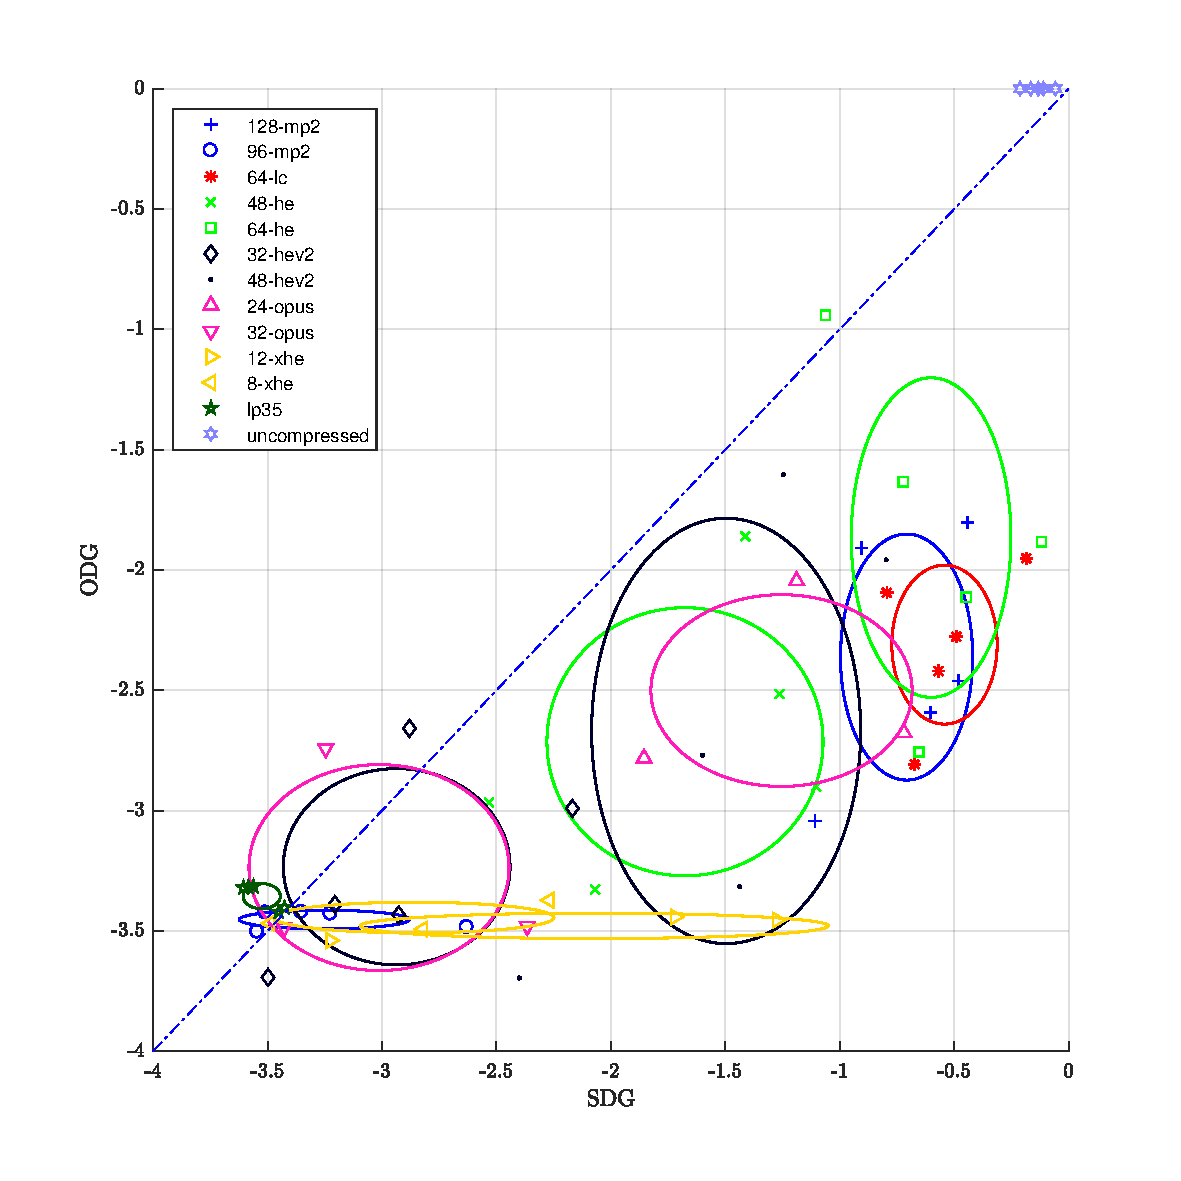
\includegraphics[width=1\linewidth]{pic/compareAdvanced.pdf}
        \caption{PEAQ Advanced}
        \label{fig:compare:advanced}
    \end{subfigure}%
    \begin{subfigure}{.5\textwidth}
        \centering
        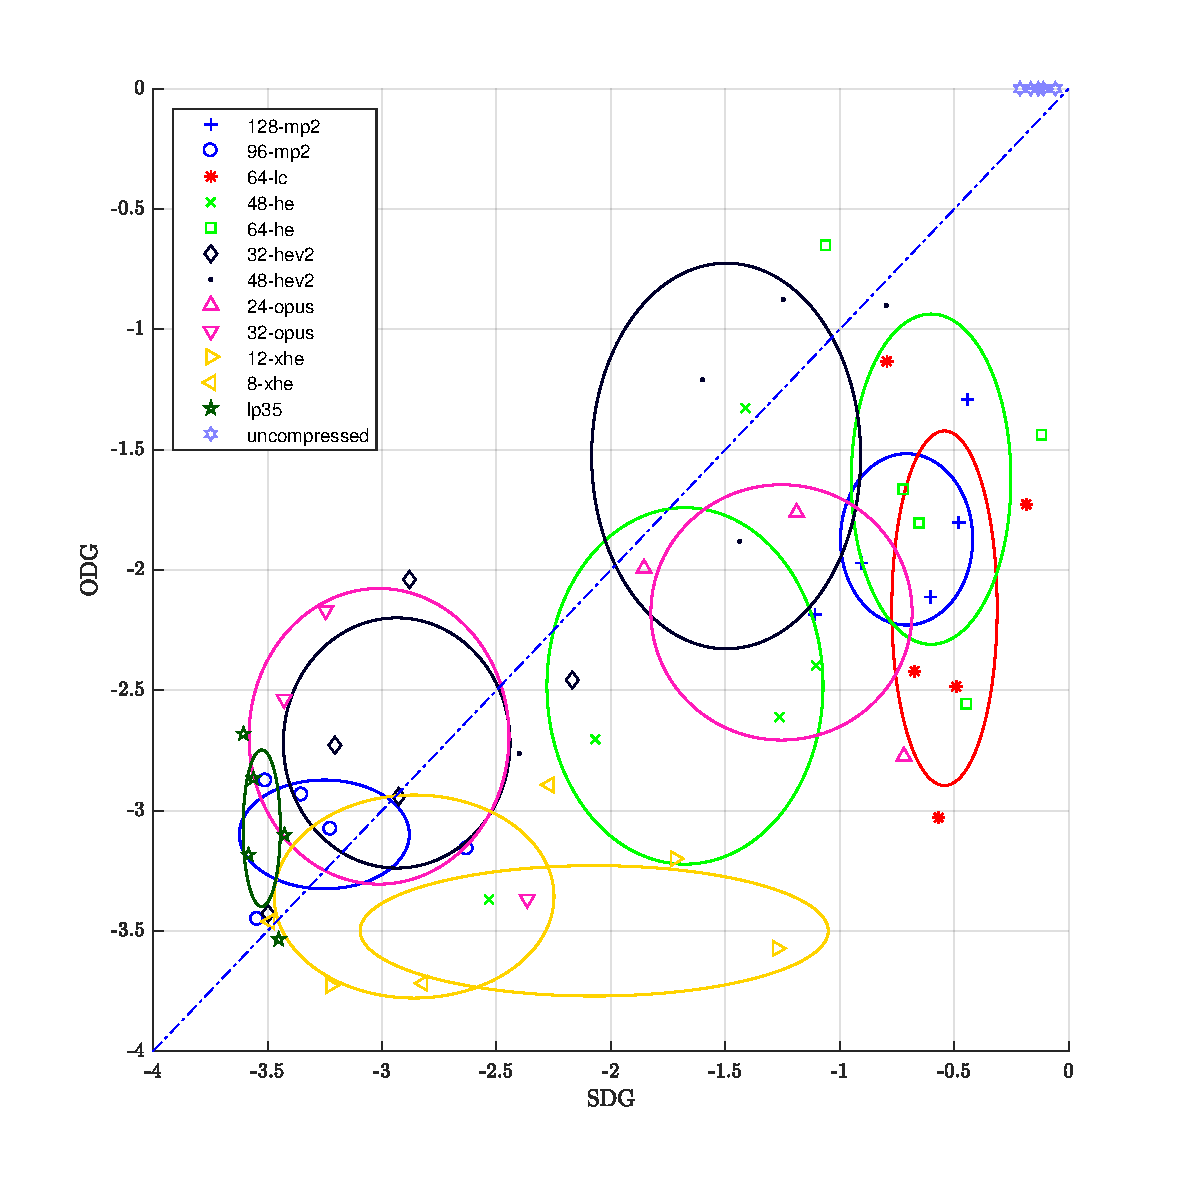
\includegraphics[width=1\linewidth]{pic/compareBasic.pdf}
        \caption{PEAQ Basic}
        \label{fig:compare:basic}
    \end{subfigure}
    \\
        \begin{subfigure}{.5\textwidth}
        \centering
        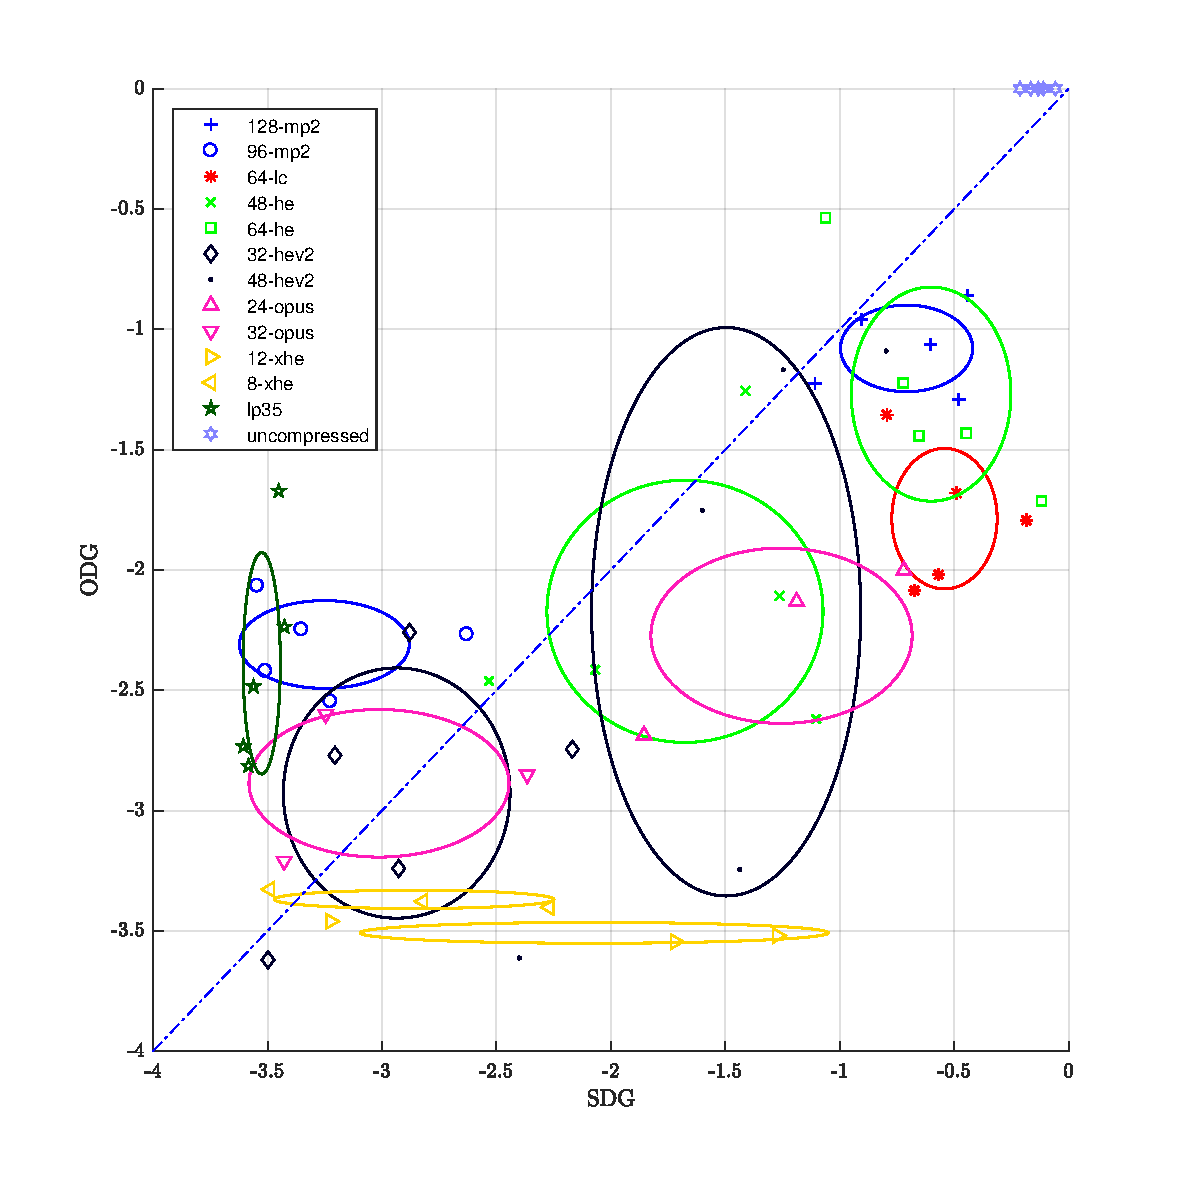
\includegraphics[width=1\linewidth]{pic/comparePemoq.pdf}
        \caption{PEMO-Q}
        \label{fig:compare:pemoq}
    \end{subfigure}%
        \begin{subfigure}{.5\textwidth}
        \centering
        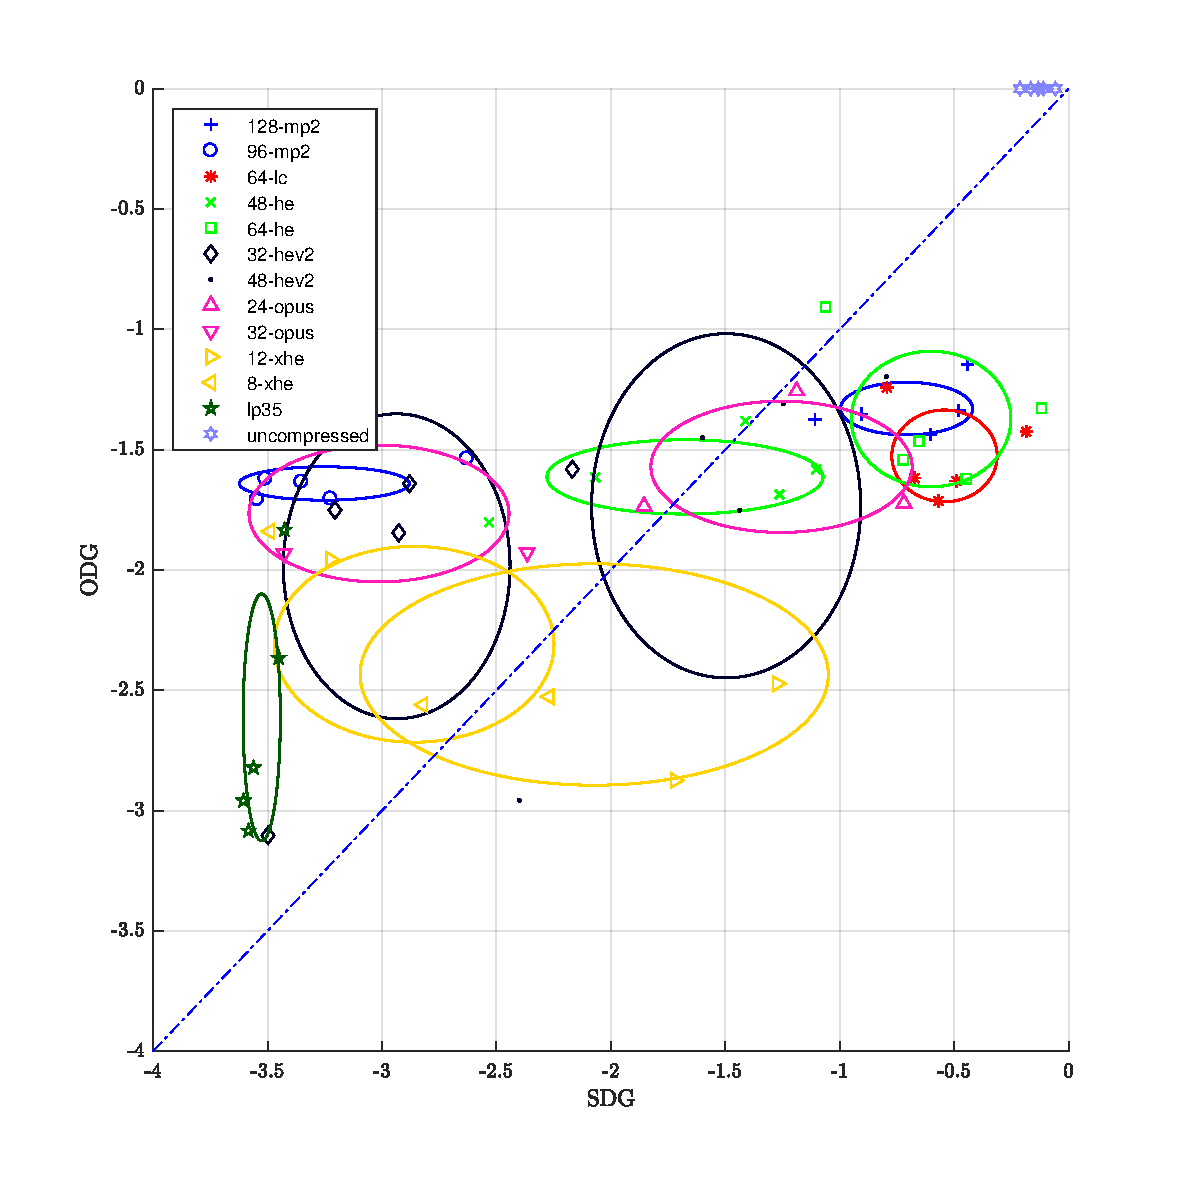
\includegraphics[width=1\linewidth]{pic/compareVisqol.pdf}
        \caption{ViSQOL}
        \label{fig:comapre:visqol}
    \end{subfigure}%
    \caption{Závislost ODG na SDG včetně oblastí vytyčených směrodatnými odchylkami objektivních a subjektivních testů}
    \label{fig:compare}
\end{figure}

Zjednodušeně řečeno, tabulka \ref{table:epsilon} říká, jak moc se jednotlivé algoritmy \uv{mýlí} a tabulka \ref{table:sigma} ukazuje, jak moc náhodné výsledky poskytují.

Bráno podle stáří, hodnocení vzorků zkomprimovaných kodekem MPEG Layer II dosahuje nízkých hodnot rozptylu přes různé druhy nahrávek. Na nižší použité rychlosti 96 kb/s hodnotí s nejmenší chybou oba zástupci algoritmu PEAQ. U PEMO-Q došlo k nadhodnocení o jeden stupeň $ODG$ a u algoritmu ViSQOL je tato hodnota ještě vyšší. Jak už bylo řečeno, MPEG Layer II se při nízkých rychlostech chová jako dolní propust, která mění spektrogram (současně tedy i neurogram) jen nepatrně, díky čemuž je \uv{políčková podobnost} vyšší než u modernějších kompresních metod. PEAQ a na něm založené PEMO-Q zřejmě přikládá vetší váhu gammatónovým filtrům modelu ucha na vysokých kmitočtech, a tak hodnotí \textit{mp2} věrněji. Na druhou stranu při vyšší bitové rychlosti je kvalita MPEG Layer II podhodnocena právě algoritmem PEAQ. Nejmenší chybu poskytl PEMO-Q a druhou nejmenší ViSQOL.

Základní profil AAC LC tvoří v grafech \ref{pic:res:Visqol} zastoupen jen jednou oblastí o bitové rychlosti 64 kb/s, kterou obě verze algoritmu PEAQ podhodnotili o více než jeden stupeň na ODG škále. Základní verze má navíc ze všech algoritmů jednoznačně nejvyšší rozptyl. Nejkonzistentnější výsledek a zároveň nejmenší chybu poskytl ViSQOL. 

Pokud se k základnímu profilu AAC přidá rozšíření SBR, projevuje se to poklesem kvadratické chyby a současným vzrůstem směrodatné odchylky u všech metod. Tento trend dál pokračuje i s poklesem rychlosti HE-AAC v1 na 48 kb/s, kromě hodnocení algoritmu ViSQOL u kterého rozptyl naopak klesá. Také chybu udává nejmenší a to $\varepsilon = 0,48$.

Dalším generačním krokem k HE-AAC v2 kvadratická chyba roste u algoritmů PEAQ a PEMO-Q, zatímco u hodnocení metodou ViSQOL chyba opět klesá. U tohoto profilu je nejvyšší rozptyl objektivně změřené kvality. Směrodatná odchylka výsledků algoritmu PEAQ dosahuje téměř 1,2 stupně ODG na obě strany od průměru. PEAQ Advanced poskytuje hodnotu $\sigma = 0,88$ a ViSQOL $\sigma = 0,72$. Oblast s nižší rcyhlostí 32 kb/s HE-AAC v2 protíná ideální převodní křivku ve třech případech ze čtyř. Jen hodnocení algoritmem ViSQOL je vyšší než u subjektivních testů a to o jeden stupeň ODG.

Kodek Opus v digitálních rádiích nefiguruje a proto jeho hodnocení nemá vliv na jakýkoliv výsledný verdikt. Na nižší rychlosti 24 kb/s ho s nejmenší chybou hodnotil algoritmus PEMO-Q a při vyšším toku 32 kb/s ViSQOL, který dosáhl taktéž nejmenší směrodatné odchylky u obou rychlostí.

Téměř zázračně nízké hodnoty směrodatné odchylky u kodeku xHE-AAC jsou způsobeny spíše tím, že PEAQ ani PEMO-Q si s jeho hodnocením neví příliš rady a tak všem testovaným vzorkům přiřadili hodnotu $ODG \approx 3,5$. Jediný ViSQOL dosahuje hodnocení, které se přibližuje výsledkům subjektivních testů.

Trochu mimo dosavadní výběr stojí dvě poslední oblasti a to skrytá kotva a skrytá reference. Jsou ovšem součástí výstupu subjektivního testování a není důvod nezařadit je do těchto závislostí po bok kompresních metod. Referenční vzorek všechny algoritmy ohodnotily bez jakékoliv ztráty kvality a tak se eliptická oblast zjednodušila na úsečku v pravém horním rohu grafů \ref{pic:res:Visqol}. Signál s potlačenými kmitočty od 3,5 kHz výše stejně jako posluchači ohodnotily obě verze algoritmu PEAQ. ViSQOL i PEMO-Q skrytou kotvu nadhodnocují zhruba o jeden stupeň ODG.

Ani jedna z metod neposkytuje ideální výsledky. Lze ale vysledovat trend, že algoritmy PEAQ a PEMO-Q poskytují horší výsledky u modernějších kodeků používaných v digitálních rádiích zatímco ViSQOL má problémy spíše s nadhodnocováním vzorků, které postrádají vyšší harmonické. ViSQOL také v průměru hodnotí s nejmenší kvadratickou chybou, což je ještě výraznější u průměrné hodnoty $\varepsilon_{radio}$, ve které jsou zahrnuty kodeky používané v DRM(+) a DAB/DAB+. Na základě těchto poznatků je označen za nejobjektivnější hodnotící metodu ze všech prezentovaných.

\section{Výsledky objektivních testů}

V zadání této práce je mimo jiné zmíněno, že vybraná objektivní metoda by měla být využita pro vyhodnocení kvality zvuku v systémech digitálního rozhlasového vysílání. Z algoritmizačního hlediska bylo jednodušší vyhodnotit kvalitu všemi metodami, pro všechny kodeky a všechny možné bitové rychlosti a naimportovat je pomocí skriptu \code{makeCell} do zobrazovacího nástroje \code{showResults}. Protože v předchozí podkapitole je jako nejvěrohodnější objektivní metoda vybrán ViSQOL, potažmo jeho varianta ViSQOLAudio jsou v tomto textu tedy vybrány pouze závislosti vygenerované algoritmem ViSQOL. 

Výsledky z ostatních algoritmů jsou k nahlédnutí v dodatku \ref{app:3}, či v samotném nástroji \code{showResults}, kde si může uživatel výstup libovolně nakonfigurovat a exportovat do souboru.

Obrázek \ref{pic:res:Visqol} obsahuje šestici grafů zobrazující průměrné $ODG$ a směrodatnou odchylku všech vzorků z tabulky \ref{table:material}. Do nich jsou rovněž vyneseny výsledky poslechových testů pro lepší představu toho jak spolu korespondují. Pro DRM+ a DAB+ jsou klíčové grafy \ref{fig:vis:sub1} a  \ref{fig:vis:sub3} až \ref{fig:vis:sub6}.

Pro hodnocení \textit{MPEG Layer II} není ViSQOL příliš vhodný avšak to je jediný případ, kdy je radno sáhnout po jiné objektivní metodě. Na velmi nízkých bitových rychlostech stále uděluje hodnocení MOS-LQO vyšší než 3, slovně řečeno lepší než přijatelné. Tento kodek je ovšem v současnosti nahrazován pokročilejšími kompresními metodami a tam si ViSQOL vede podstatně lépe.

Podobně jako první subjektivní test ukázal, že mezi generacemi HE-AAC v1 a HE-AAC v2 lidské ucho téměř neslyší rozdíl, hodnotí v průměru ViSQOL tyto dva profily velmi podobně. U HE-AAC v2 nicméně podává výsledky se zhruba o třetinu větším rozptylem. Užití rozšíření PS a SBR má své výhody, ale i rizika. S rostoucím bitovým tokem se kódový zisk nabytý použitím metod založených na psychoakustických poznatcích klesá a v určitém momentu již nastoupí výhody nižšího profilu.

\begin{figure}[H]
    \centering
    \begin{subfigure}{.5\textwidth}
        \centering
        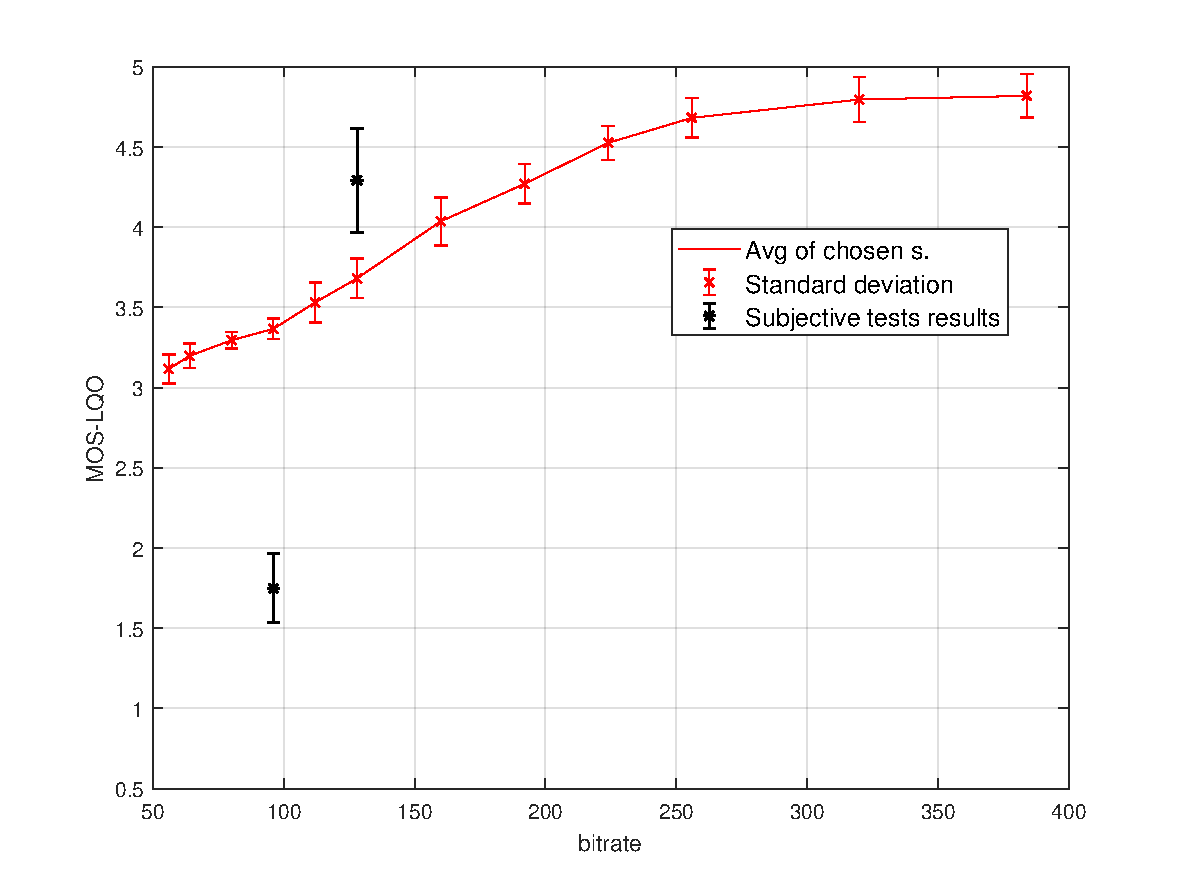
\includegraphics[width=1\linewidth]{pic/objective/mp2Visqol.pdf}
        \caption{MP2}
        \label{fig:vis:sub1}
    \end{subfigure}%
    \begin{subfigure}{.5\textwidth}
        \centering
        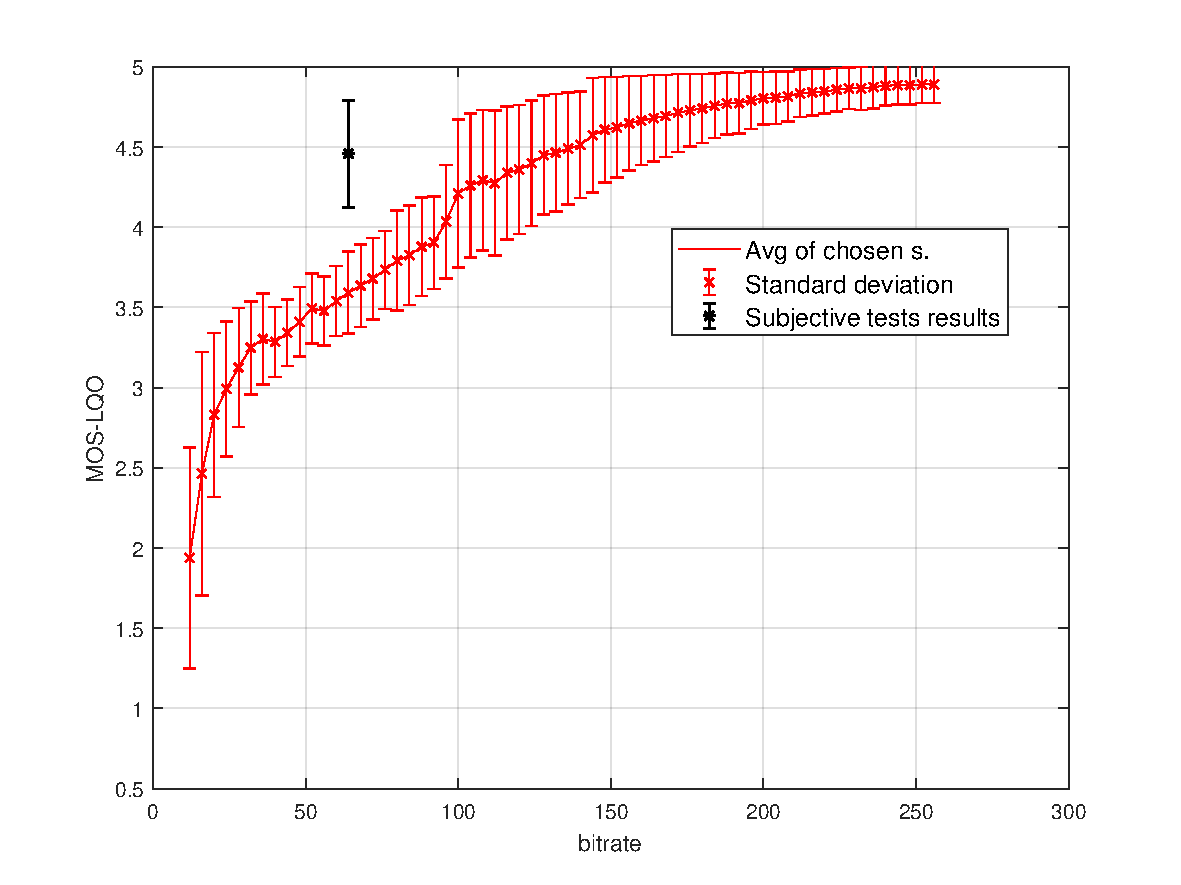
\includegraphics[width=1\linewidth]{pic/objective/lcVisqol.pdf}
        \caption{LC-AAC}
        \label{fig:vis:sub2}
    \end{subfigure}
    \\
%\end{figure}
%\begin{figure}[htb]\ContinuedFloat        
    \begin{subfigure}{.5\textwidth}
        \centering
        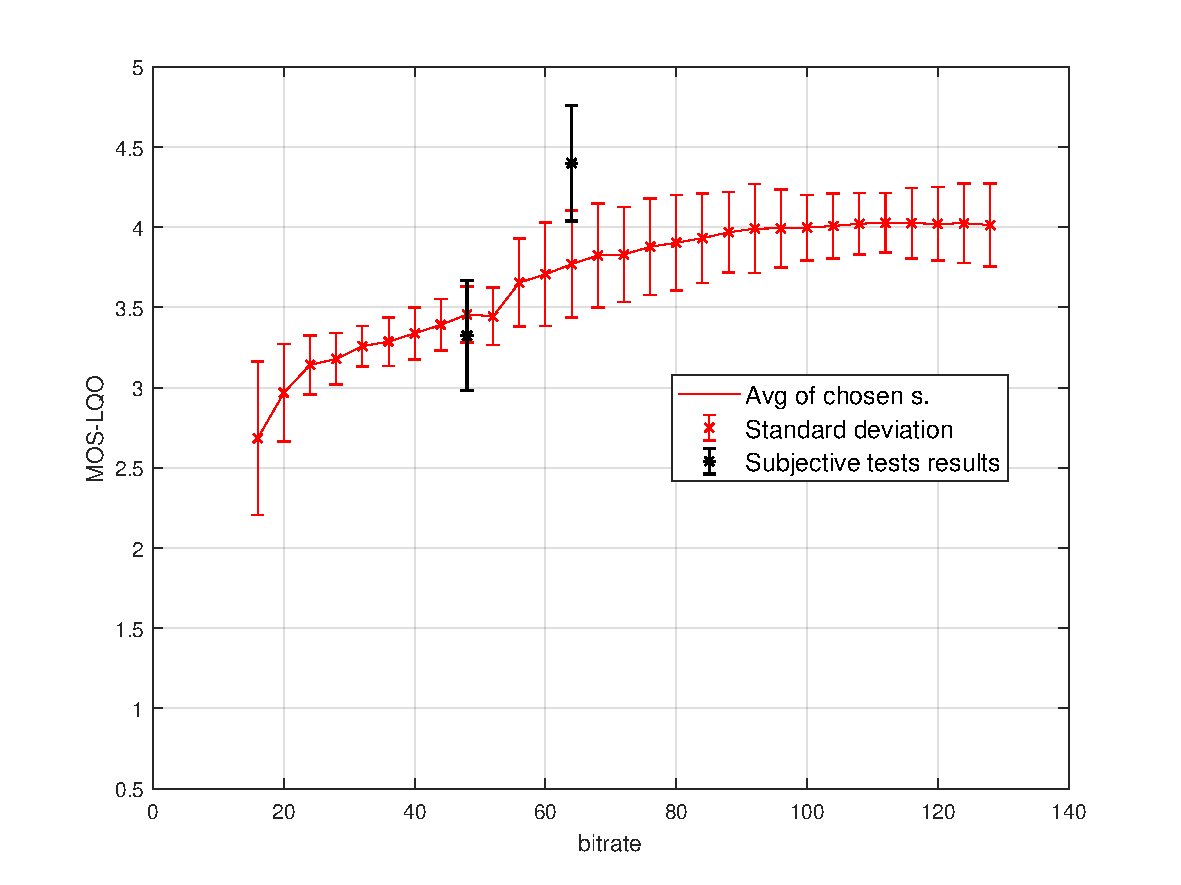
\includegraphics[width=1\linewidth]{pic/objective/heVisqol.pdf}
        \caption{HE-AAC v1}
        \label{fig:vis:sub3}
    \end{subfigure}%
        \begin{subfigure}{.5\textwidth}
        \centering
        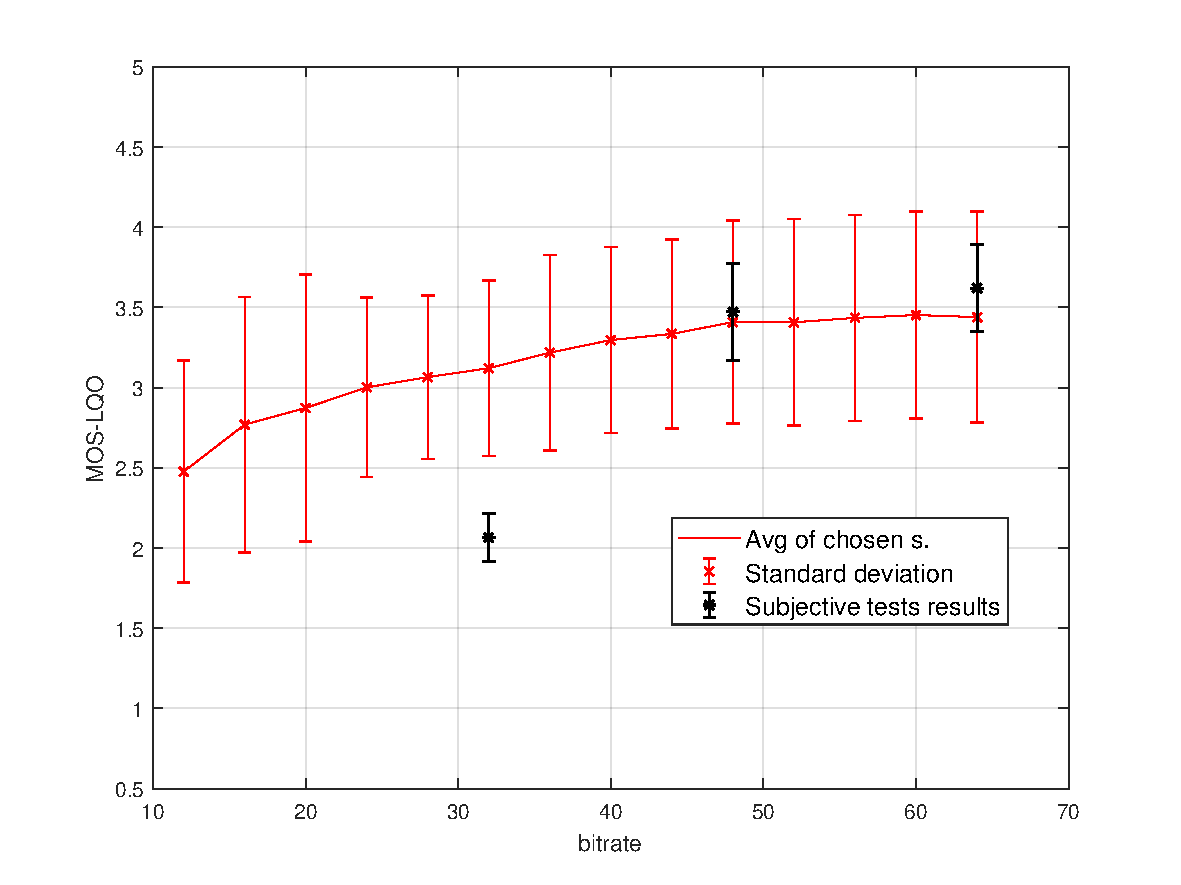
\includegraphics[width=1\linewidth]{pic/objective/hev2Visqol.pdf}
        \caption{HE-AAC v2}
        \label{fig:vis:sub4}
    \end{subfigure}%
    \\
\end{figure}
\begin{figure}[h]\ContinuedFloat
        \begin{subfigure}{.5\textwidth}
        \centering
        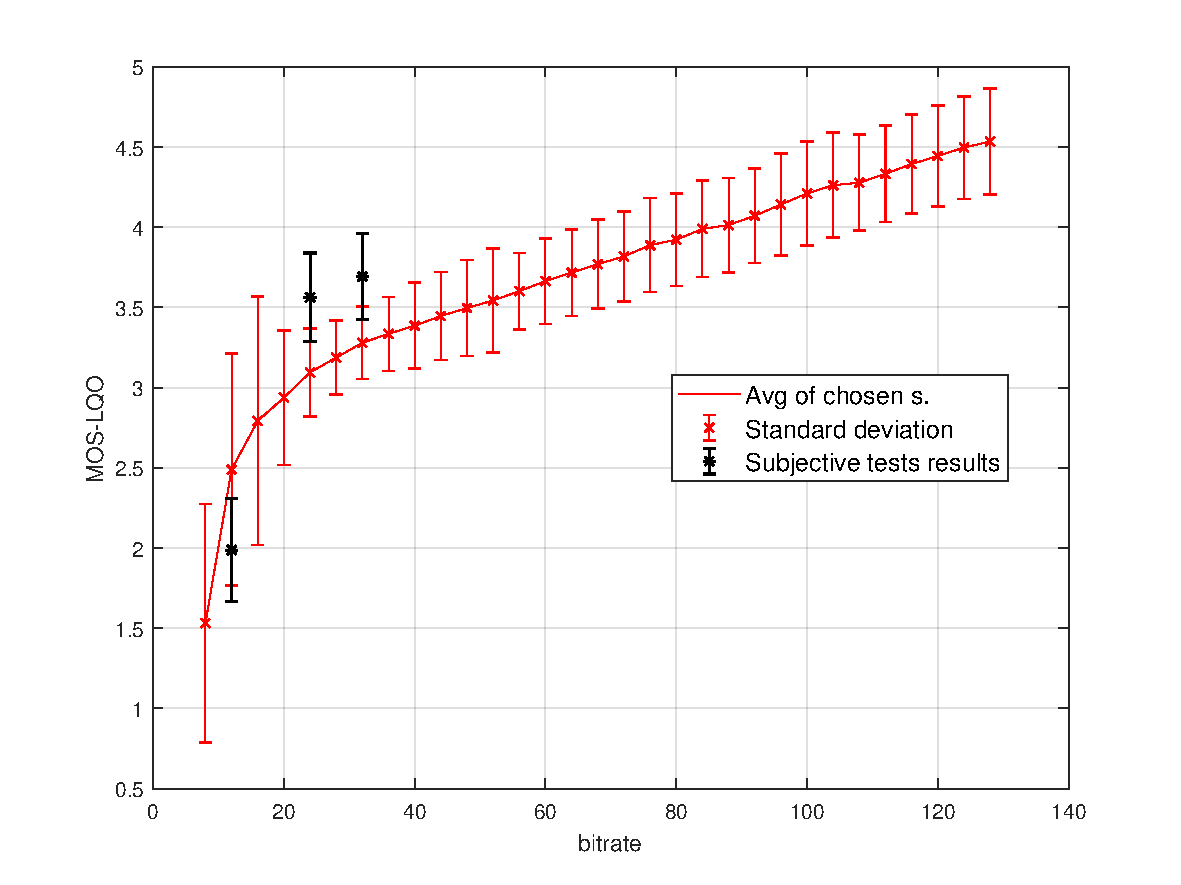
\includegraphics[width=1\linewidth]{pic/objective/opusVisqol.pdf}
        \caption{Opus}
        \label{fig:vis:sub5}
    \end{subfigure}%
        \begin{subfigure}{.5\textwidth}
        \centering
        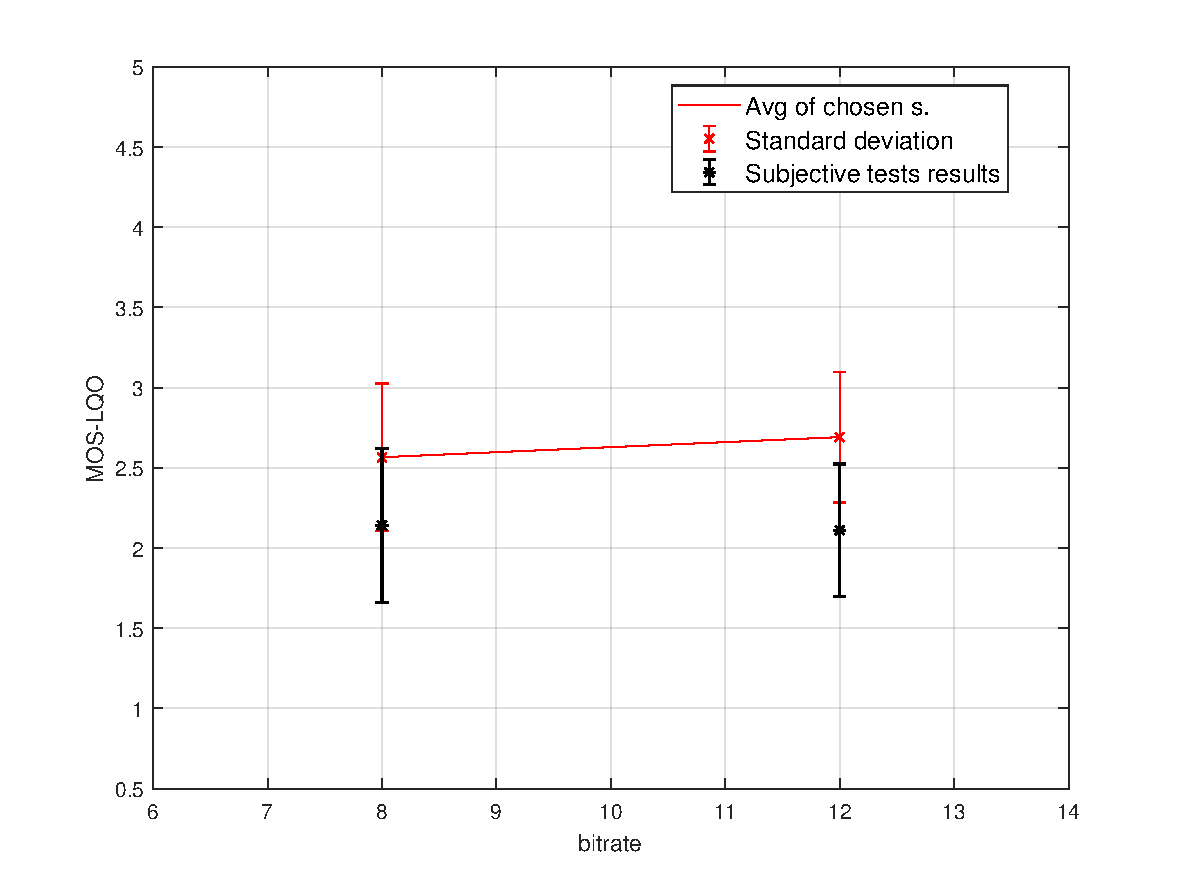
\includegraphics[width=1\linewidth]{pic/objective/xheVisqol.pdf}
        \caption{xHE-AAC}
        \label{fig:vis:sub6}
    \end{subfigure}%
    \caption{Hodnocení algoritmem ViSQOL.} 
\label{pic:res:Visqol}
\end{figure}

\bigskip
\bigskip

I přes to, že k rozhodnutí zvolit právě ViSQOL nevedlo hodnocení vzorků zakódovaných kodekem Opus, je podobnost objektivních a subjektivních výsledků značná.

%Lze očekávat, že v blízké budoucnosti bude svět DRM postupně adaptován na využití kodeku xHE-AAC, který nabízí přijatelnou kvalitu na velmi nízkých rychlostech. Jak si stojí při použití vyšší bitové rychlosti 

Ze závislostí na obrázku \ref{pic:res:Visqol} lze říci, že pokud má být kvalita zvuku přenášeného digitálním rádiem hodnocena posluchači jako vynikající nezbývá než volit z kodeků MPEG Layer II a AAC LC. U prvního ze zmíněných je třeba bitového toku 160 kb/s či více, druhému k překročení spodní hranice vynikající kvality stačí 128 kb/s. Žádná jiná z kompresních metod tohoto kvalitativního prahu nedosahuje. 

Pokud je poskytovatel ochotný slevit ze svých požadavků a vysílat kvalitou označovanou jako dobrá (60 \% - 80 \% na CQS stupnici), dosáhne nejvyšší efektivity volbou profilu HE-AAC v2 na bitové rychlosti 44 kb/s. Kdyby z nějakých důvodů nebylo možné využít rozšíření \textit{Parametric Stereo}, dosáhne stejného výsledku s bitovým tokem 56 kb/s profilů HE-AAC v1 a AAC LC, které na této rychlosti ViSQOL hodnotí stejně. Při použití MPEG Layer II by bylo potřeba dvojnásobného toku 112 kb/s. 

Pokud je prioritou úspora prostředků a padne rozhodnutí vysílat pouze přijatelnou kvalitou, lze dle hodnocení algoritmu ViSQOL využít kompresní metodu xHE-AAC. Pro přenos mluveného slova je dostatečnou bitovou rychlostí 8 kb/s. Při přenosu hudebních záznamů je lepší sáhnout po rychlosti 12 kb/s. Jaké kvality xHE-AAC dosahuje na vyšších tocích bohužel kvůli absenci kodéru nebylo zjištěno. V digitálním rádiu DAB, které xHE-AAC neintegruje lze stejné kvality pro vysílání řeči dosáhnout užitím kodeku HE-AAC v2 s tokem 16 kb/s a pro přenos hudebního obsahu nejméně 20 kb/s.



